\section*{Anhang}
\label{sec:anhang}
\addcontentsline{toc}{section}{Anhang}

\label{fig:webinterface_screenshots}

\begin{figure}[H]
    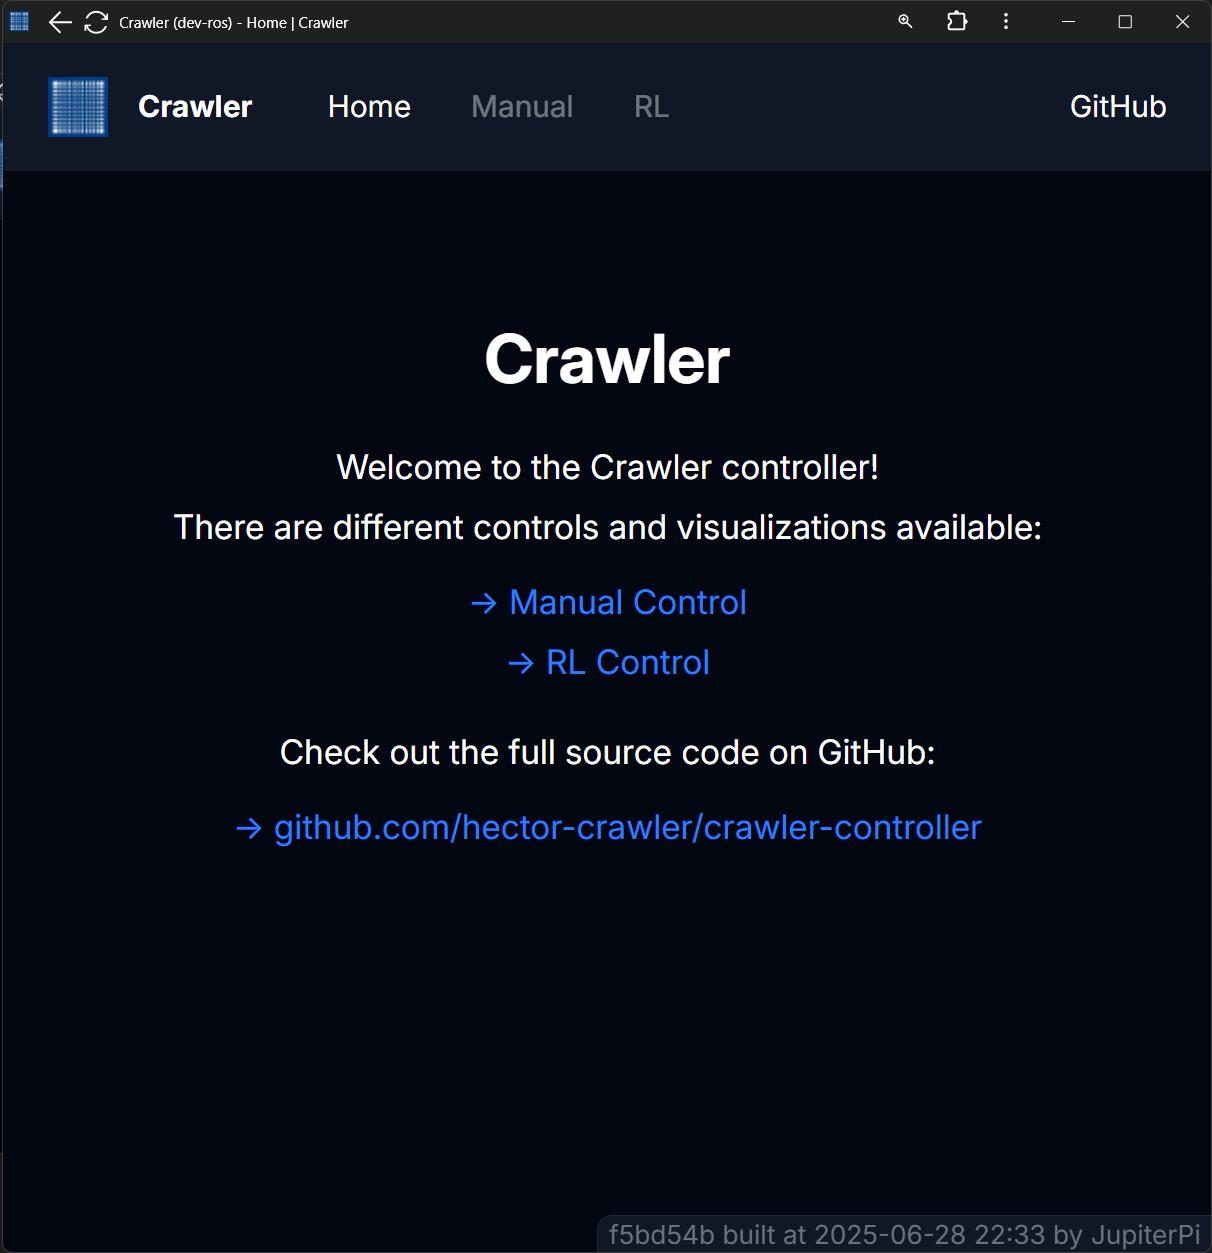
\includegraphics[width=0.5\textwidth]{photos/webinterface_home.png}
    \caption{Webinterface-Seite \texttt{/home} mit einleitenden Informationen und weiterführenden Links}
\end{figure}

\begin{figure}[H]
	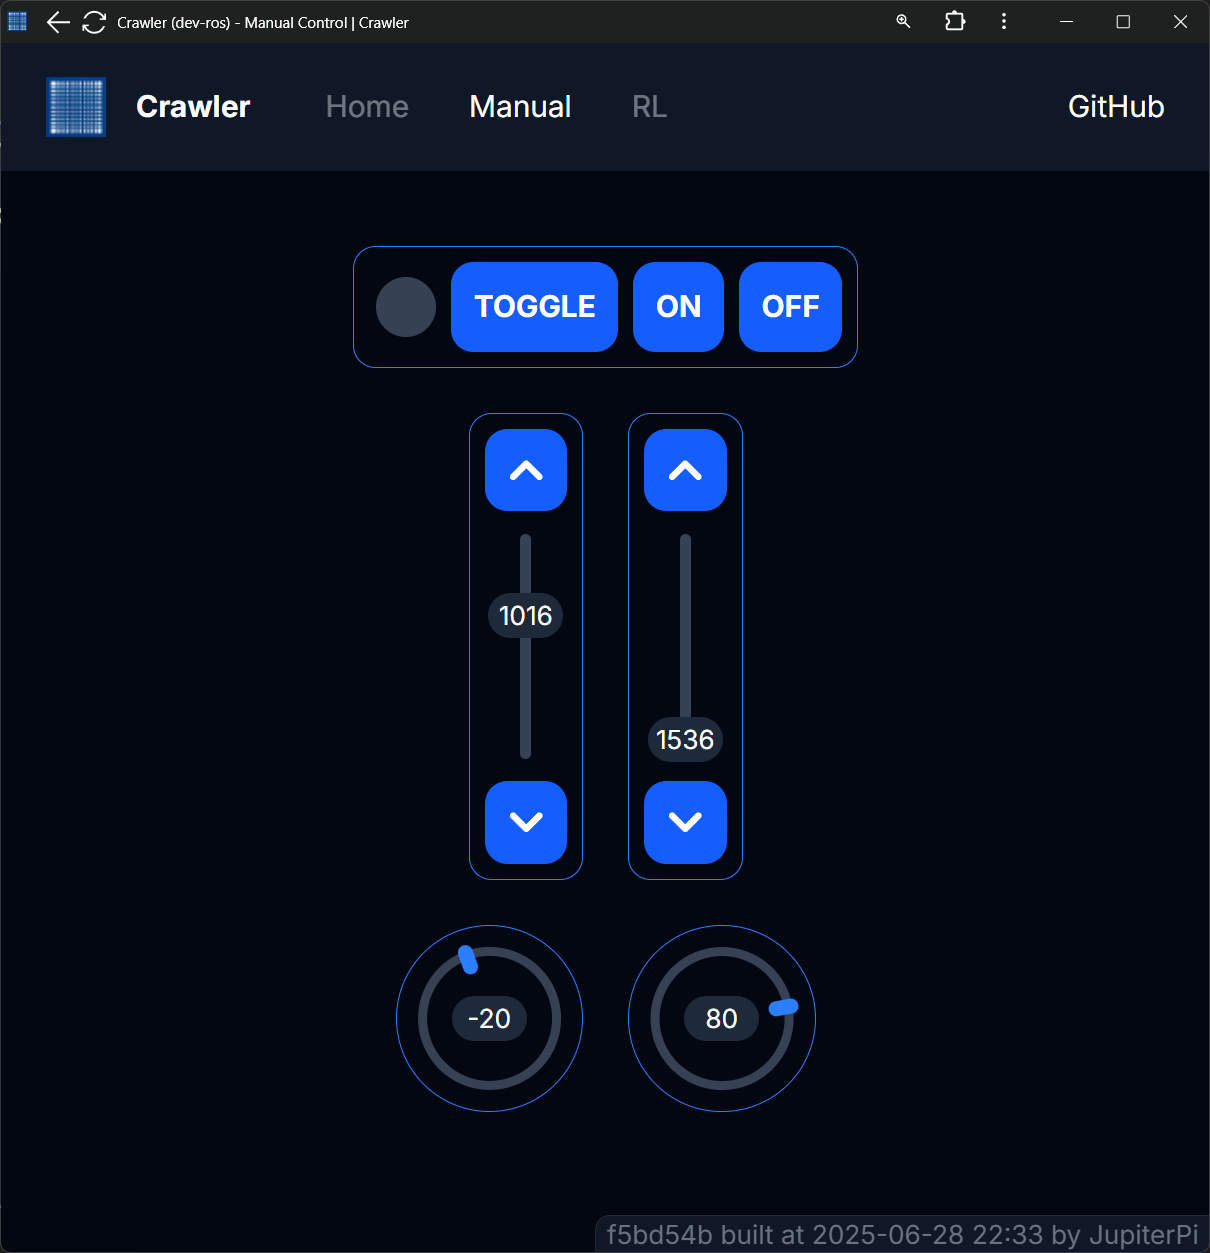
\includegraphics[width=0.7\textwidth]{photos/webinterface_manualControl.png}
    \caption{Webinterface-Seite \texttt{/manualControl} zur manuellen Kontrolle und Anzeige der Hardwarekomponenten}
\end{figure}

\begin{figure}[H]
	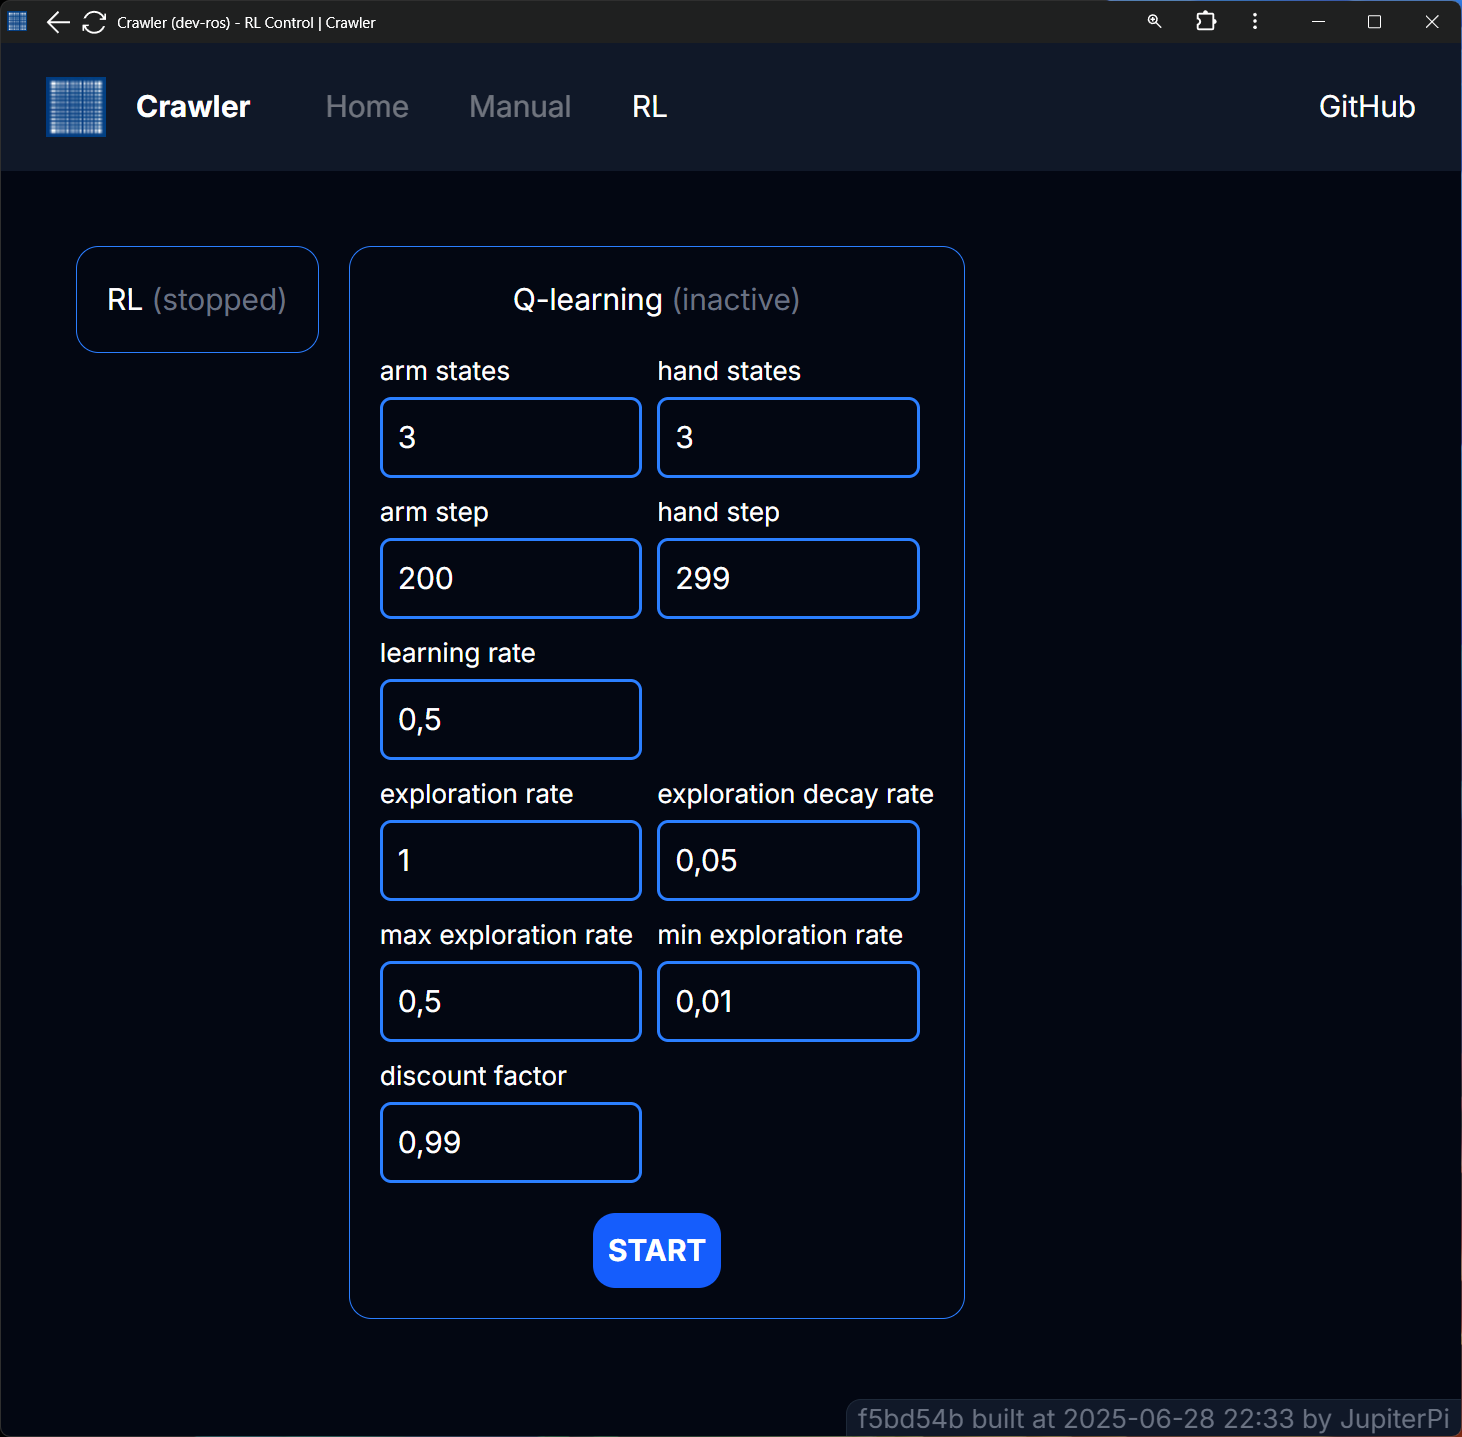
\includegraphics[scale=0.22]{photos/webinterface_rlControl_1.png}
	\caption{Webinterface-Seite \texttt{/rlControl} zur Konfiguration der Parameter des Q-Learning}
\end{figure}

\begin{figure}[H]
	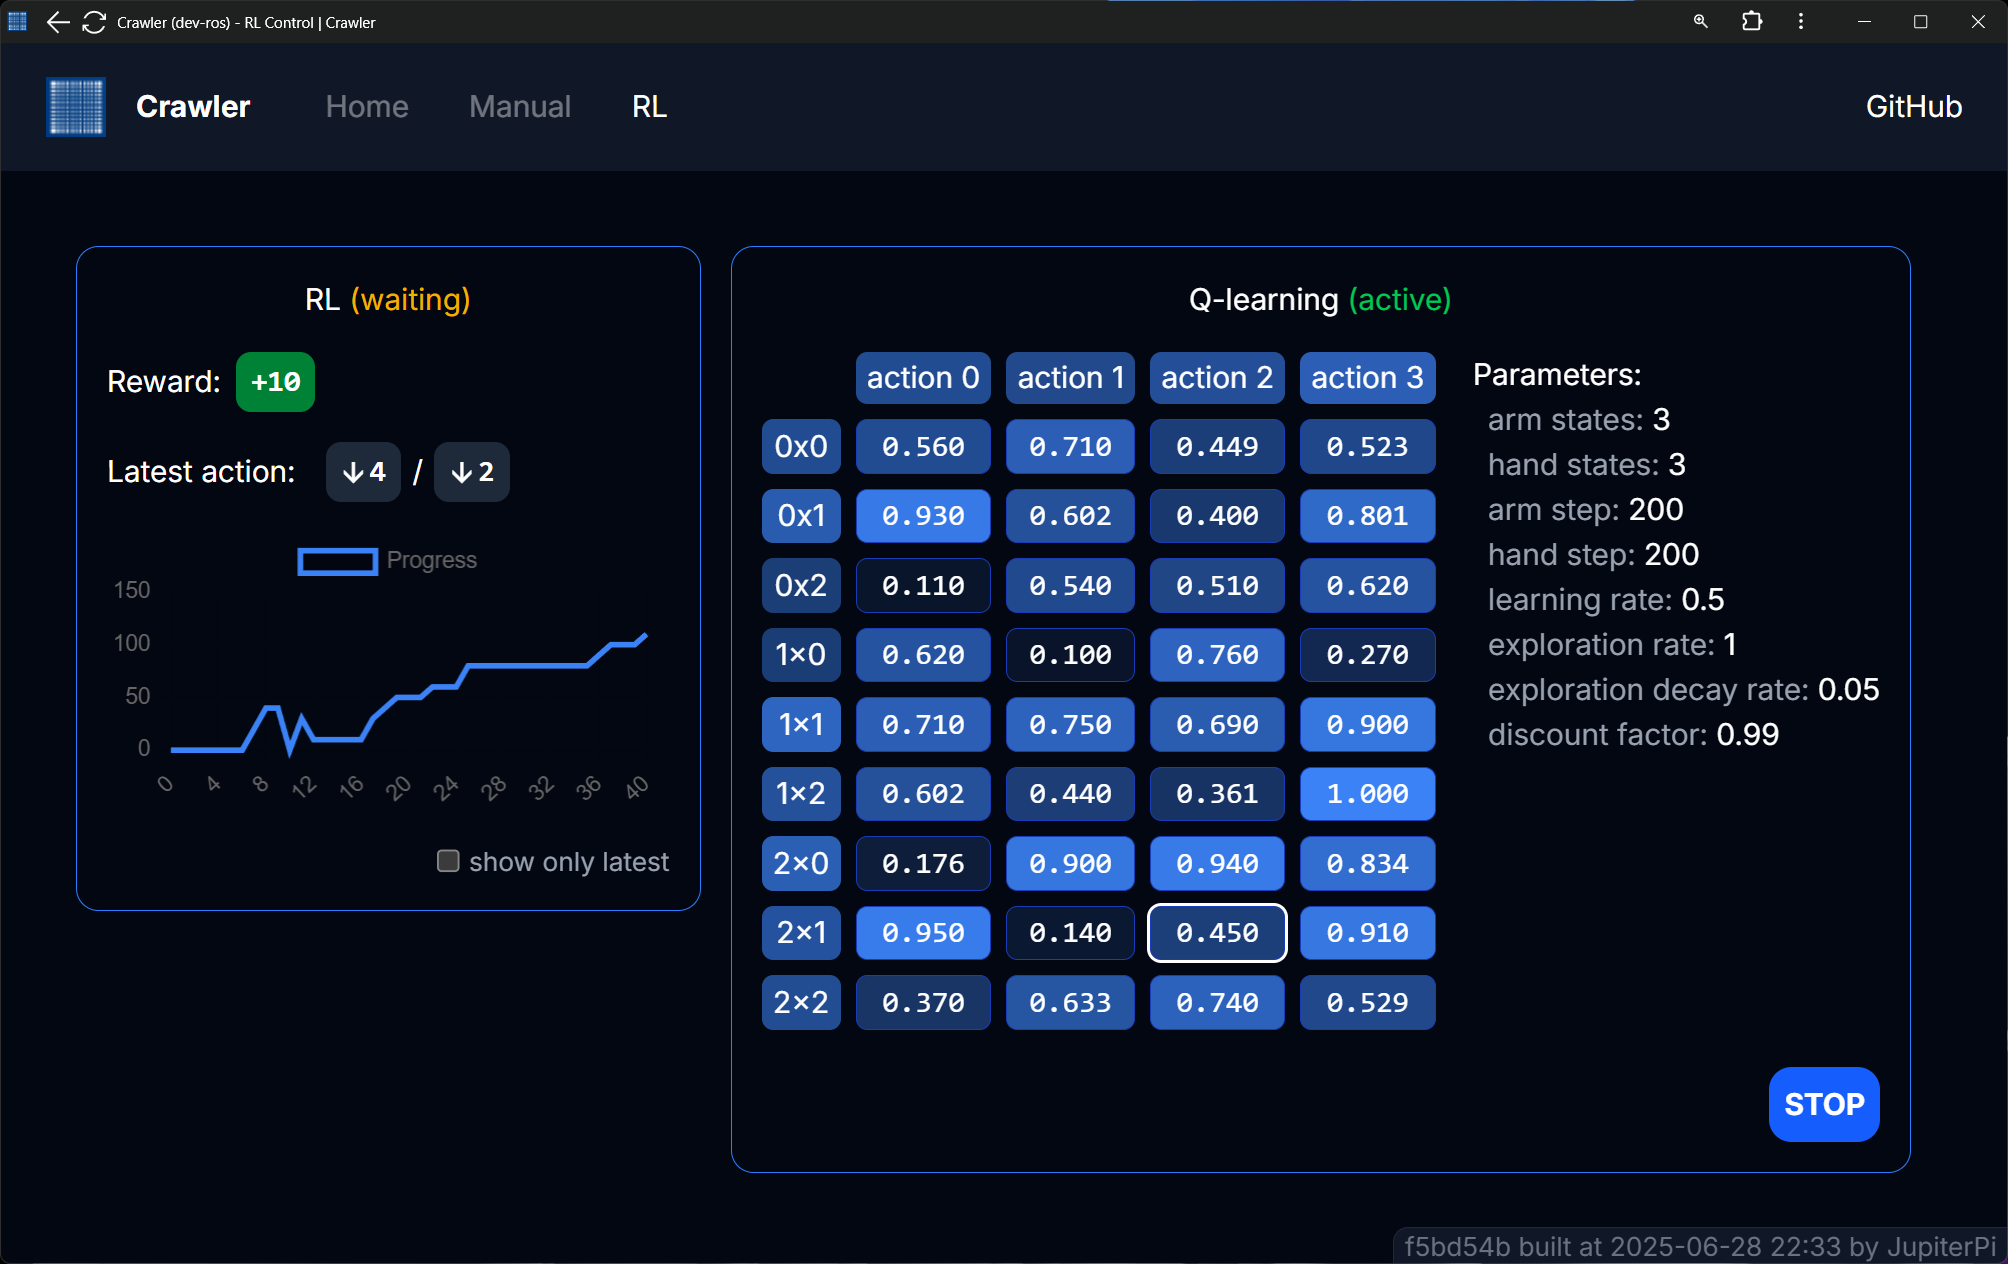
\includegraphics[width=\textwidth]{photos/webinterface_rlControl_2.png}
	\caption{Webinterface-Seite \texttt{/rlControl} nach dem Starten, mit Visualisierungen des RL-Environments (links) und der Q-Table (rechts)}
\end{figure}

%%%%

\section*{Quellen}
\addcontentsline{toc}{section}{Quellen}
\bib
\appendix

\newcommand{\selbststaendigkeitserklaerung}[1]{
	\newpage
	\section*{Selbstständigkeitserklärung}
	Hiermit versichere ich, {#1}, dass ich diese Arbeit unter der Beratung durch Herrn Prof. Dr. Ihme selbstständig verfasst habe und keine anderen als die angegebenen Quellen und Hilfsmittel benutzt wurden, sowie Zitate kenntlich gemacht habe. \\[2cm]

	Ort, Datum \hfill \rule{5cm}{0.4pt} \\
	\hfill (Unterschrift)
}

\selbststaendigkeitserklaerung{Gregor Niehl}
\selbststaendigkeitserklaerung{Jonathan Kraus}
\selbststaendigkeitserklaerung{Pascal Roth}
